% ------------------------------------------------------------------------
% ------------------------------------------------------------------------
% Modelo UFSC para Trabalhos Academicos (tese de doutorado, dissertação de
% mestrado) utilizando a classe abntex2
%
% Autor: Alisson Lopes Furlani
% 	Modificações:
%	- 27/08/2019: Alisson L. Furlani, add pacote 'glossaries' para listas
%   - 06/11/2019: Luiz-Rafael Santos, modifica para Trabalho de Conclusão de Curso
% ------------------------------------------------------------------------
% ------------------------------------------------------------------------

\documentclass[
	% -- opções da classe memoir --
	12pt,				% tamanho da fonte
	%openright,			% capítulos começam em pág ímpar (insere página vazia caso preciso)
	oneside,			% para impressão no anverso. Oposto a twoside
	a4paper,			% tamanho do papel. 
	% -- opções da classe abntex2 --
	chapter=TITLE,		% títulos de capítulos convertidos em letras maiúsculas
	section=TITLE,		% títulos de seções convertidos em letras maiúsculas
	%subsection=TITLE,	% títulos de subseções convertidos em letras maiúsculas
	%subsubsection=TITLE,% títulos de subsubseções convertidos em letras maiúsculas
	% -- opções do pacote babel --
	english,			% idioma adicional para hifenização
	%french,				% idioma adicional para hifenização
	%spanish,			% idioma adicional para hifenização
	brazil				% o último idioma é o principal do documento
	]{abntex2}

\usepackage{setup/ufscthesisA4-alf}

% ---
% Filtering and Mapping Bibliographies
% ---
% Pacotes de citações
% ---
\usepackage{csquotes}
\usepackage[backend = biber, style = abnt]{biblatex}
\usepackage{xstring}
\usepackage{listings}
%\usepackage{natbib}
% FIXME Se desejar estilo numérico de citações,  comente a linha acima e descomente a linha a seguir.
% \usepackage[backend = biber, style = numeric-comp]{biblatex}

\lstset{
    frame=single,
    columns=flexible,
    basicstyle={\small\ttfamily},
}

\setlength\bibitemsep{\baselineskip}
\DeclareFieldFormat{url}{Disponível~em:\addspace\url{#1}}
\NewBibliographyString{sineloco}
\NewBibliographyString{sinenomine}
\DefineBibliographyStrings{brazil}{%
	sineloco     = {\mkbibemph{S\adddot l\adddot}},
	sinenomine   = {\mkbibemph{s\adddot n\adddot}},
	andothers    = {\mkbibemph{et\addabbrvspace al\adddot}},
	in			 = {\mkbibemph{In:}}
}

\addbibresource{aftertext/references.bib} % Seus arquivos de referências

% ---
\DeclareSourcemap{
	\maps[datatype=bibtex]{
		% remove fields that are always useless
		\map{
			\step[fieldset=abstract, null]
			\step[fieldset=pagetotal, null]
		}
		% remove URLs for types that are primarily printed
%		\map{
%			\pernottype{software}
%			\pernottype{online}
%			\pernottype{report}
%			\pernottype{techreport}
%			\pernottype{standard}
%			\pernottype{manual}
%			\pernottype{misc}
%			\step[fieldset=url, null]
%			\step[fieldset=urldate, null]
%		}
		\map{
			\pertype{inproceedings}
			% remove mostly redundant conference information
			\step[fieldset=venue, null]
			\step[fieldset=eventdate, null]
			\step[fieldset=eventtitle, null]
			% do not show ISBN for proceedings
			\step[fieldset=isbn, null]
			% Citavi bug
			\step[fieldset=volume, null]
		}
	}
}
% ---

% ---
% Informações de dados para CAPA e FOLHA DE ROSTO
% ---
% FIXME Substituir 'Nome completo do autor' pelo seu nome.
\autor{Maria Joaquina}
% FIXME Substituir 'Título do trabalho' pelo título da trabalho.
\titulo{Comparação de compiladores da linguagem de programação C para plataforma WebAssembly}
% FIXME Substituir 'Subtítulo (se houver)' pelo subtítulo da trabalho.  
% Caso não tenha substítulo, comente a linha a seguir.
% \subtitulo{Subtítulo (se houver)}
% FIXME Substituir 'XXXXXX' pelo nome do seu
% orientador.
\orientador{Prof. Zé de Maria Preá, Me.}
% FIXME Se for orientado por uma mulher, comente a linha acima e descomente a linha a seguir.
% \orientador[Orientadora]{Nome da orientadora, Dra.}
% FIXME Substituir 'XXXXXX' pelo nome do seu
% coorientador. Caso não tenha coorientador, comente a linha a seguir.
% \coorientador{Prof. XXXXXX, Dr.}
% FIXME Se for coorientado por uma mulher, comente a linha acima e descomente a linha a seguir.
% \coorientador[Coorientadora]{XXXXXX, Dra.}
% FIXME Substituir 'XXXXXX' pelo nome do Coordenador do 
% programa/curso.
\coordenador{Prof. Maria Bernadete, Me.}
% FIXME Se for coordenadora mulher, comente a linha acima e descomente a linha a seguir.
% \coordenador[Coordenadora]{Nome da Coordenadora, Dra.}
% FIXME Substituir '[ano da entrega]' pelo ano (ano) em que seu trabalho foi defendido.
\ano{2023}
% FIXME Substituir '[dia] de [mês] de [ano]' pela data em que ocorreu sua defesa.
\data{18 de dezembro de 2023}
% FIXME Substituir '[Cidade da defesa]' pela cidade em que ocorreu sua defesa.
\local{Salgueiro - PE}
\instituicaosigla{UNIVASF}
\instituicao{Universidade Federal do Vale do São Francisco}
% FIXME Substituir 'Dissertação/Tese' pelo tipo de trabalho (Tese, Dissertação). 
\tipotrabalho{Trabalho de Conclusão de Curso}
% FIXME Substituir '[licenciado/bacharel] em [nome do título obtido]' pela grau adequado.
\formacao{Bacharel em Ciência da Computação}
% FIXME Substituir '[licenciado/bacharel]' pelo nivel adequado.
\nivel{bacharel}
% FIXME Substituir 'Curso de Graduação em [XXXXXXXX]' pela curso adequado.
\programa{Bacharelado em Ciência da Computação}
% FIXME Substituir 'Campus XXXXXX ou Centro de XXXXXX' pelo campus ou centro adequado.
\centro{Campus Salgueiro - PE}
\preambulo
{%
\imprimirtipotrabalho~do curso de \imprimirprograma~apresentado ao Colegiado de Ciência da Computação como requisito parcial para obtenção do título de \imprimirformacao.
}
% ---

% ---
% Configurações de aparência do PDF final
% ---
% alterando o aspecto da cor azul
\definecolor{blue}{RGB}{41,5,195}
% informações do PDF
\makeatletter
\hypersetup{
     	%pagebackref=true,
		pdftitle={\@title}, 
		pdfauthor={\@author},
    	pdfsubject={\imprimirpreambulo},
	    pdfcreator={LaTeX with abnTeX2},
		pdfkeywords={ufsc, latex, abntex2}, 
		colorlinks=true,       		% false: boxed links; true: colored links
    	linkcolor=black,%blue,          	% color of internal links
    	citecolor=black,%blue,        		% color of links to bibliography
    	filecolor=black,%magenta,      		% color of file links
		urlcolor=black,%blue,
		bookmarksdepth=4
}
\makeatother
% ---

% ---
% compila a lista de abreviaturas e siglas e a lista de símbolos
% ---

% Declaração das siglas
\siglalista{HTML}{Linguagem de Marcação de Texto (do inglês, \textit{HyperText Markup Language})}
\siglalista{HTML5}{HTML versão 5}
\siglalista{JS}{JavaScript}
\siglalista{Wasm}{WebAssembly}
\siglalista{WAT}{WebAssembly Text}
\siglalista{WABT}{Kit de Ferramentas para Binário WebAssembly (do inglês, \textit{WebAssembly Binary Toolkit})}
\siglalista{VM}{Máquina virtual (do inglês, \textit{Virtual Machine})}
\siglalista{WWW}{Rede Mundial de Computadores (do inglês, \textit{World Wide Web})}
\siglalista{W3C}{Consórcio da Rede Mundial de Computadores (do inglês, \textit{World Wide Web Consortium})}
\siglalista{CSV}{Valores Separados por Vírgula (do inglês, \textit{Comma Separated Values})}
\siglalista{GCC}{GNU Compiler Collection}
\siglalista{LTS}{Suporte de Longo Termo (do inglês, \textit{Long Term Support})}
\siglalista{WASI}{WebAssembly System Interface}

% Declaração dos simbolos
\simbololista{C}{\ensuremath{C}}{Circunferência de um círculo}
\simbololista{pi}{\ensuremath{\pi}}{Número pi} 
\simbololista{r}{\ensuremath{r}}{Raio de um círculo}
\simbololista{A}{\ensuremath{A}}{Área de um círculo}

% compila a lista de abreviaturas e siglas e a lista de símbolos
\makenoidxglossaries 

% ---

% ---
% compila o indice
% ---
\makeindex
% ---

% ----
% Início do documento
% ----
\begin{document}

% Seleciona o idioma do documento (conforme pacotes do babel)
%\selectlanguage{english}
\selectlanguage{brazil}

% Retira espaço extra obsoleto entre as frases.
\frenchspacing 

% Espaçamento 1.5 entre linhas
\OnehalfSpacing

% Corrige justificação
%\sloppy

% ----------------------------------------------------------
% ELEMENTOS PRÉ-TEXTUAIS
% ----------------------------------------------------------
% \pretextual %a macro \pretextual é acionado automaticamente no início de \begin{document}
% ---
% Capa, folha de rosto, ficha bibliografica, errata, folha de apróvação
% Dedicatória, agradecimentos, epígrafe, resumos, listas
% ---
% ---
% Capa
% ---
\imprimircapa
% ---

% ---
% Folha de rosto
% (o * indica que haverá a ficha bibliográfica)
% ---
\imprimirfolhaderosto*
% ---

% ---
% Inserir a ficha bibliografica
% ---
% http://ficha.bu.ufsc.br/
\begin{fichacatalografica}
	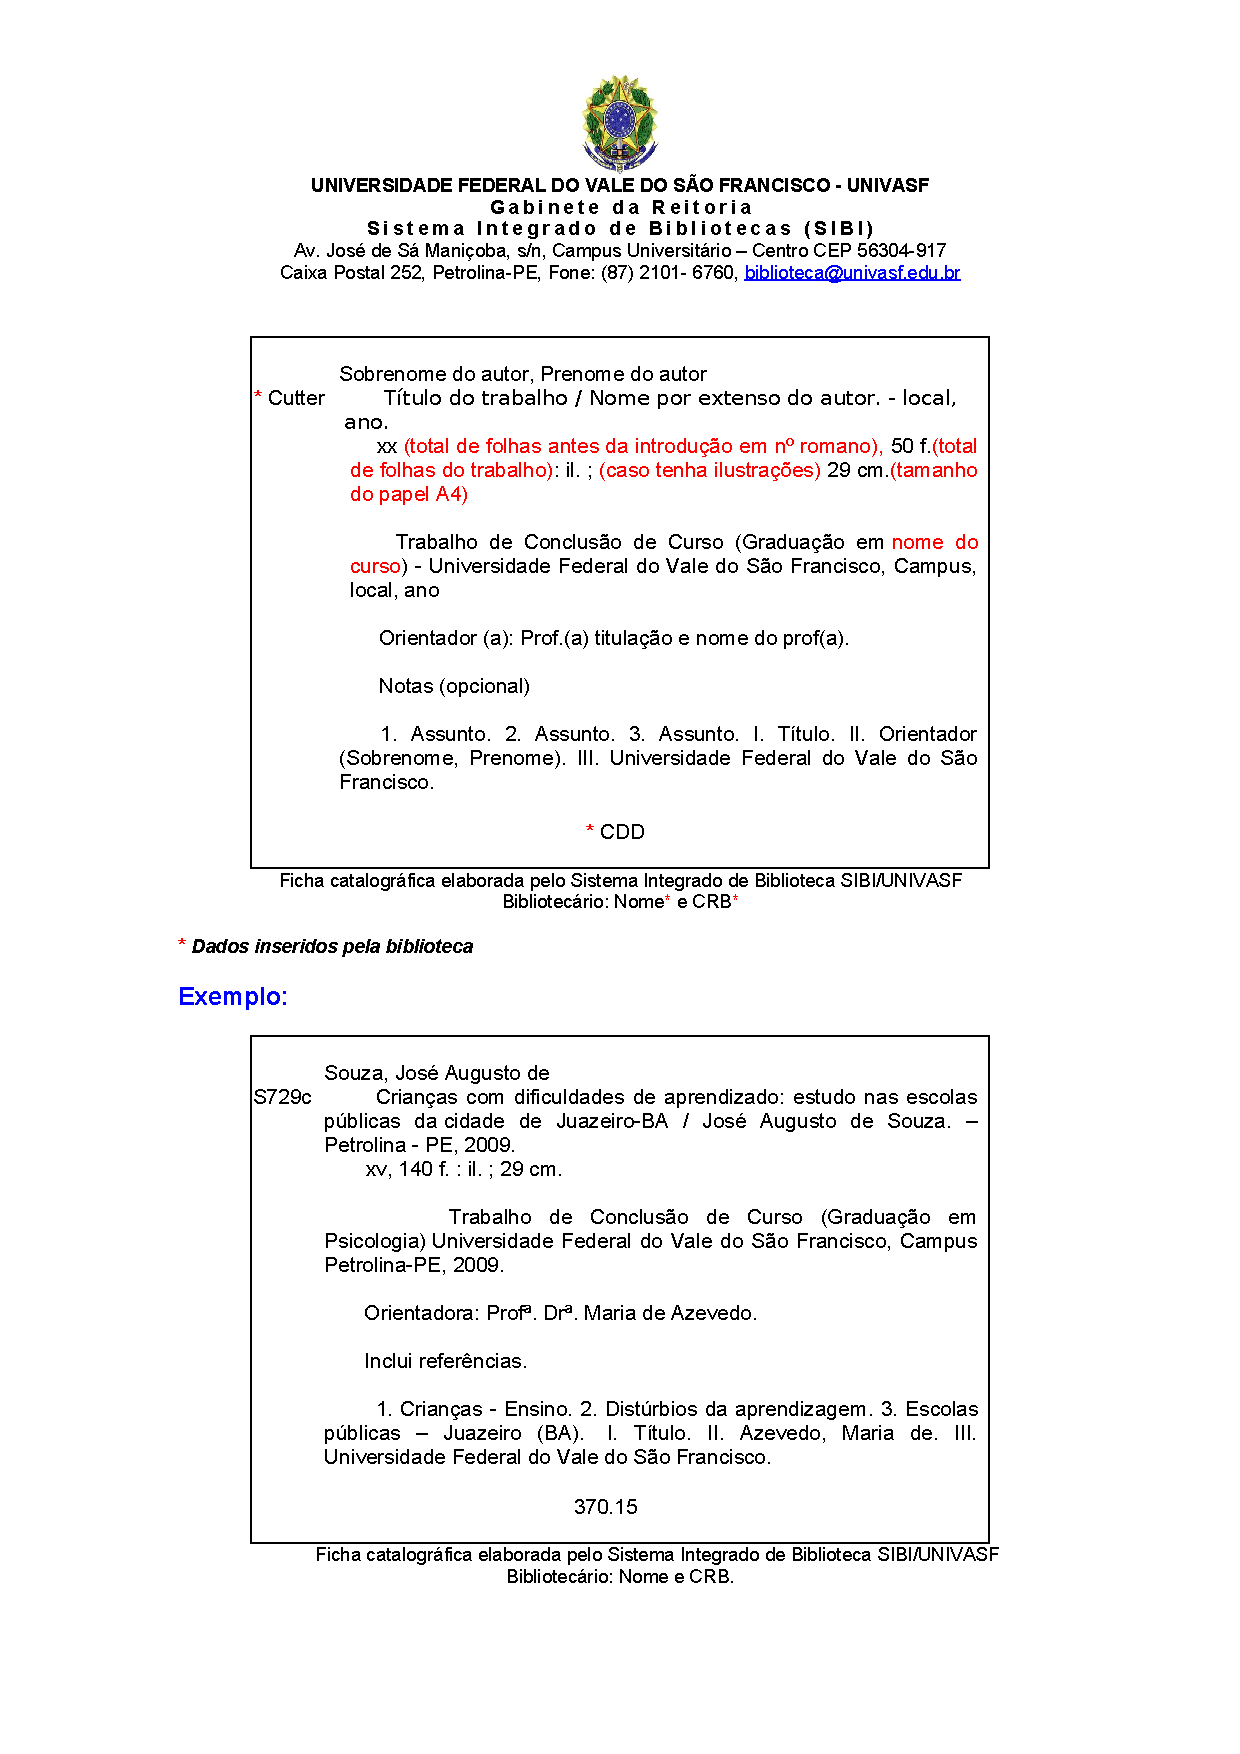
\includepdf{beforetext/ficha-catalografica-tcc.pdf}
\end{fichacatalografica}
% ---

\setlength{\ABNTEXsignwidth}{10cm}

% ---
% Inserir folha de aprovação
% ---
\begin{folhadeaprovacao}
	\OnehalfSpacing
	\centering
	\imprimirautor\\%
	\vspace*{10pt}		
	\textbf{\imprimirtitulo}%
	\ifnotempty{\imprimirsubtitulo}{:~\imprimirsubtitulo}\\%
	%		\vspace*{31.5pt}%3\baselineskip
	\vspace*{\baselineskip}
	%\begin{minipage}{\textwidth}
	% ~do~\imprimirprograma~do~\imprimircentro~da~\imprimirinstituicao~para~a~obtenção~do~título~de~\imprimirformacao.
	Este~\imprimirtipotrabalho~foi julgado adequado para obtenção do título de \imprimirformacao~e aprovado em sua forma final pela banca examinadora. \\
		\vspace*{\baselineskip}
	\imprimirlocal, \imprimirdata. \\
	\vspace*{2\baselineskip}
	\assinatura{\OnehalfSpacing\imprimircoordenador \\ \imprimircoordenadorRotulo~do Curso}
	\vspace*{2\baselineskip}
	\textbf{Banca Examinadora:} \\
	\vspace*{\baselineskip}
	\assinatura{\OnehalfSpacing\imprimirorientador \\ Presidente da Banca}
	%\end{minipage}%
	\vspace*{\baselineskip}
	\assinatura{Prof. X Y Z, Me.\\
	Avaliador \\
	\imprimirinstituicao}

	\vspace*{\baselineskip}
	\assinatura{Prof. X Y Z, Dr.\\
	Avaliador \\
	\imprimirinstituicao}


\end{folhadeaprovacao}
% ---

% ---
% Dedicatória
% ---
%\begin{dedicatoria}
%	\vspace*{\fill}
%	\noindent
%	\begin{adjustwidth*}{}{5.5cm}     
%		Este trabalho é dedicado aos meus colegas de classe e aos meus queridos pais.
%	\end{adjustwidth*}
%\end{dedicatoria}
% ---

% ---
% Agradecimentos
% ---
\begin{agradecimentos}

Agradeço a meu pai, minha mãe, meu cachorro, minha sogra e por último e menos importante, meu orientador.
\end{agradecimentos}
% ---

% ---
% Epígrafe
% ---
%\begin{epigrafe}
%	\vspace*{\fill}
%	\begin{flushright}
%		\textit{``Texto da Epígrafe.\\
%			Citação relativa ao tema do trabalho.\\
%			É opcional. A epígrafe pode também aparecer\\
%			na abertura de cada seção ou capítulo.\\
%			Deve ser elaborada de acordo com a NBR 10520.''\\
%			(Autor da epígrafe, ano)}
%	\end{flushright}
%\end{epigrafe}
% ---

% ---
% RESUMOS
% ---

% resumo em português
\setlength{\absparsep}{18pt} % ajusta o espaçamento dos parágrafos do resumo
\begin{resumo}
	\SingleSpacing
Lorem Ipsum is simply dummy text of the printing and typesetting industry. Lorem Ipsum has been the industry's standard dummy text ever since the 1500s, when an unknown printer took a galley of type and scrambled it to make a type specimen book. It has survived not only five centuries, but also the leap into electronic typesetting, remaining essentially unchanged. It was popularised in the 1960s with the release of Letraset sheets containing Lorem Ipsum passages, and more recently with desktop publishing software like Aldus PageMaker including versions of Lorem Ipsum.


	\textbf{Palavras-chave}: WebAssembly. Web. Desempenho. Compiladores. Emscripten. Cheerp.
\end{resumo}

% resumo em inglês
\begin{resumo}[Abstract]
	\SingleSpacing
	\begin{otherlanguage*}{english}


Lorem Ipsum is simply dummy text of the printing and typesetting industry. Lorem Ipsum has been the industry's standard dummy text ever since the 1500s, when an unknown printer took a galley of type and scrambled it to make a type specimen book. It has survived not only five centuries, but also the leap into electronic typesetting, remaining essentially unchanged. It was popularised in the 1960s with the release of Letraset sheets containing Lorem Ipsum passages, and more recently with desktop publishing software like Aldus PageMaker including versions of Lorem Ipsum.

		
		\textbf{Keywords}: WebAssembly. Web. Performance. Compilers. Emscripten. Cheerp.
	\end{otherlanguage*}
\end{resumo}

%% resumo em francês 
%\begin{resumo}[Résumé]
% \begin{otherlanguage*}{french}
%    Il s'agit d'un résumé en français.
% 
%   \textbf{Mots-clés}: latex. abntex. publication de textes.
% \end{otherlanguage*}
%\end{resumo}
%
%% resumo em espanhol
%\begin{resumo}[Resumen]
% \begin{otherlanguage*}{spanish}
%   Este es el resumen en español.
%  
%   \textbf{Palabras clave}: latex. abntex. publicación de textos.
% \end{otherlanguage*}
%\end{resumo}
%% ---

{%hidelinks
	\hypersetup{hidelinks}
	% ---
	% inserir lista de ilustrações
	% ---
	\pdfbookmark[0]{\listfigurename}{lof}
	\listoffigures*
	\cleardoublepage
	% ---
	
	% ---
	% inserir lista de quadros
	% ---
	\pdfbookmark[0]{\listofquadrosname}{loq}
	\listofquadros*
	\cleardoublepage
	% ---
	
	% ---
	% inserir lista de tabelas
	% ---
	\pdfbookmark[0]{\listtablename}{lot}
	\listoftables*
	\cleardoublepage
	% ---
	
	% ---
	% inserir lista de abreviaturas e siglas (devem ser declarados no preambulo)
	% ---
	\imprimirlistadesiglas
	% ---
	
	% ---
	% inserir lista de símbolos (devem ser declarados no preambulo)
	% ---
	\imprimirlistadesimbolos
	% ---
	
	% ---
	% inserir o sumario
	% ---
	\pdfbookmark[0]{\contentsname}{toc}
	\tableofcontents*
	\cleardoublepage
	
}%hidelinks
% ---

% ---

% ----------------------------------------------------------
% ELEMENTOS TEXTUAIS
% ----------------------------------------------------------
\textual

% ---
% 1 - Introdução
% ---
% ----------------------------------------------------------
\chapter{Introdução}\label{cap1}
% ----------------------------------------------------------

No início da Rede Mundial de Computadores, os sites eram compostos principalmente de simples documentos na \Gls{HTML}, com pouca lógica, dinamicidade e interatividade. Para trazer dinamicidade e outras funcionalidades, a indústria convergiu para o uso da linguagem de programação \Gls{JS} \cite{rise_of_js}. No entanto, com a popularização da Internet, e da necessidade de páginas mais complexas, surge o desejo de utilizar novas tecnologias que poderiam superar o JS em alguns aspectos, sendo a performance o principal aspecto desejado, dentre estas ferramentas, são notáveis: asm.js e \Gls{Wasm} \cite{wasm_predecessors}.

\section{Questões de Pesquisa}

O desenvolvimento desse trabalho foi elaborado com objetivo de responder as seguintes questões de pesquisa:

\begin{description}
    \item[QP01] Qual dos dois compiladores estudados emite um binário com tamanho menor?
    \item[QP02] Entre os dois, qual produz um binário que utiliza menos memória, considerando o tamanho inicial da memória igual para ambos?
    \item[QP03] Entre ambos, qual produz um binário com tempo de execução menor?
\end{description}

\section{Objetivos}

Os objetivos deste trabalho são subdivididos em objetivos gerais e objetivos específicos. Estes são:

\subsection{Objetivo Geral}

Realizar comparação entre os compiladores Emscripten e Cheerp considerando o tamanho do binário emitido pelas duas ferramentas, a quantidade de memória utilizada pelo binário, e o tempo de execução em diferentes \textit{browsers}.

\subsection{Objetivos Específicos}

Os objetivos específicos são:

\begin{itemize}
    \item Compilar para WebAssembly os algoritmos do \textit{benchmark} Polybench/C\cite{polybench}, permitindo que os binários finais sejam utilizados para comparar a performance dos compiladores Emscripten e Cheerp.
    \item Comparar o tamanho do binário resultante de cada compilador ao compilar os algoritmos do Polybench/C.
    \item Executar no Google Chrome e Firefox cada algoritmo compilado para WebAssembly, capturar e analisar o uso de memória e tempo de execução de cada um dos algoritmos.
\end{itemize}

\section{Justificativa}

A execução deste trabalho torna-se justificável devido a baixa quantidade de pesquisas que realizam comparação entre as ferramentas, Emscripten e Cheerp. Há também textos de \textit{blogs} que realizam essa comparação, no entanto, o rigor cientifico não é muito presente nos mesmos, como será visto na seção de Trabalhos Correlatos, \ref{correlatos}.

\section{Organização do Trabalho}

Esse trabalho é organizado como segue: No capítulo \ref{fundamentacao} é apresentado os conceitos base para melhor entendimento das tecnologias abordadas. Portanto, o capítulo apresenta uma introdução sobre a plataforma WebAssembly, seguida por duas seções informativas sobre os dois compiladores utilizados. Ao final do capítulo é também listado as principais pesquisas relacionadas. No capítulo seguinte, \ref{delineamento}, é descrito os passos necessários para realizar o experimento desejado assim como o ambiente adotado para execução da pesquisa. No capítulo \ref{resultados} é apresentado os dados coletados no experimento executado, em seguida é feito uma análise dos dados visando responder as questões de pesquisa. Por fim, no capítulo \ref{conclusoes} é sintetizado o que foi realizado na pesquisa assim como os resultados obtidos ao final da análise de dados.




\chapter{Fundamentação Teórica}\label{fundamentacao}

Este capítulo apresenta os conceitos básicos que envolvem o tema da pesquisa, assim como descreve os trabalhos correlatos a este, para melhor entendimento do contexto em que se encontra as pesquisas em WebAssembly.

\section{WebAssembly}

Desde quando JS tornou-se padrão nos navegadores, houve a tentativa de utilizar outras linguagens e ferramentas com certas vantagens sobre JS, são exemplos Java Applets e ActiveX, ambas não são mais utilizadas nas tecnologias que formam a web moderna, \gls{HTML5}, ECMAScript standard, WebGL, entre outras \cite{wasm_predecessors}.

Com esse conceito, pode-se dinamicamente crescer a quantidade de memória disponível especificando a quantidade de páginas de memória extra que se deseja, isto pode ser feito utilizando chamada de métodos via JS, ou utilizando a instrução \code{memory.grow}, definida pela máquina virtual. Além desta instrução, há várias outras instruções que operam sobre a memória, podem ser vistas em \thiscite{meminstructions}{Webassembly Community Group}. Por fim, diferente da memória do JS, não existe coletor de lixo
\footnote{O coletor de lixo, também chamado de \textit{garbage collector}, é um mecanismo de gerenciamento de memória automático, ele monitora o uso de memória e decide quando libera-la. É uma tecnologia presente em várias linguagens de \textit{scripts}, como o próprio JS. Atualmente, a VM do WebAssembly não possui coletor de lixo, no entanto, há uma discussão aberta entre os criadores do WebAssembly para permitir a integração com o coletor de lixo do JS, a discussão pode ser vista em \href{https://github.com/WebAssembly/gc}{github.com/WebAssembly/gc}.}
nem formas de diminuir o tamanho da memória dinamicamente \cite{definitive_guide}.

\subsection{Instalação e Uso}

Para finalizar o tópico sobre este compilador, será apresentado a sua instalação e realizado a compilação do mesmo exemplo utilizado para o compilador anterior, permitindo perceber a diferença no processo de compilação das duas ferramentas e a diferença no \textit{bytecode} gerado.

\begin{quadro}
\caption{Comandos para instalação do Cheerp}
\begin{lstlisting}
sudo add-apt-repository ppa:leaningtech-dev/cheerp-ppa
sudo apt-get update
sudo apt-get install cheerp-core=3.0-1~focal
\end{lstlisting}
\label{instalacao_cheerp}
\end{quadro}

Neste exemplo, é utilizado o compilador GCC para compilar o algoritmo \code{atax}, o qual faz parte do coleção do PolyBench/C. Neste comando é utilizado o parâmetro \code{-I} duas vezes para adicionar os cabeçalhos \code{utilities/polybench.h} e \code{linear-algebra/kernels/atax/atax.h}. Por fim, é também adicionado para compilação o arquivo \code{utilities/polybench.c} que é necessário para a execução do algoritmo.

\section{Trabalhos correlatos}\label{correlatos}

A busca dos trabalhos que foram citados ou utilizados por esse pesquisa foi realizada no motor de busca Google Scholar, este foi escolhido pois seleciona trabalhos de diversas bases, o que aumenta a quantidade de resultados. Neste sistema de busca, para encontrar trabalhos correlatos foi utilizado as seguintes consultas: \code{WebAssembly Comparison} para buscar trabalhos que realizem comparações no contexto de WebAssembly; \code{Emscripten OR Cheerp} para buscar trabalhos que referenciem os compiladores utilizados nesta pesquisa.

Sobre WebAssembly, \thiscite{bringing_up}{Haas \textit{et al.}} é o documento científico que realiza o anúncio do WebAssembly e especifica suas características. Após a implementação do WebAssembly nos principais \textit{browsers}, foi realizado uma busca de diversos binários do WebAssembly para analisar a adoção da tecnologia e seus casos de uso em \thiscite{prevalence_in_wild}{Musch \textit{et al.}}. Ademais, em \thiscite{real_world_binaries}{Aaron \textit{et al.}} é expandido o estudo citado anteriormente, buscando uma quantidade maior de binários, nele é concluído que WebAssembly deixou sua infância de lado e está sendo adotado em diversos casos de uso.

As duas últimas pesquisas citadas são as principais encontradas que realizam a comparação entre os dois compiladores da linguagem C e apresentam resultados divergentes entre si, estes resultados serão utilizados como comparação aos resultados anunciados na seção \ref{resultados}. Em resumo, há muitos trabalhos relacionados que realizam comparação entre WebAssembly e outros tecnologias, sendo JS e asm.js as principais. No entanto, há poucos trabalhos comparando os compiladores disponíveis para WebAssembly \cite{c_vs_rust}.




\chapter{Delineamento Metodológico}\label{delineamento}

Nesta pesquisa foi realizado um experimento onde os dados coletados permitam comparar a performance do binário gerado por dois compiladores na plataforma WebAssembly, com isso, trata-se de uma pesquisa experimental e quantitativa \cite{metodologia}. Além disso, quanto ao seu objetivo, trata-se de uma pesquisa descritiva, pois tem o objetivo de obter dados de um experimento e descreve-los \cite{gil}.

\section{Descrição do experimento}\label{descricao_experimento}

Para realizar o experimento, foi criado \textit{scripts} escritos nas linguagens bash, Python e JS que são responsáveis por executar o experimento de forma automática. Dessa forma, o experimento pôde avançar rápido com pouca intervenção humana que poderia ocasionar erros.

\section{Captura de métricas utilizadas}\label{manipulacoes}

Nessa seção será explicado como é capturado as métricas utilizadas na pesquisa, além de explicar as decisões tomadas sobre como realizar a captura.

\begin{quadro}
\caption{Arquivo \code{cheerp\_capture\_time.js} adicionado ao código emitido pelo Cheerp}
\begin{lstlisting}
var polybench_time = null;
var initial_memory = null;
var memory_used = null;
var _log = console.log;
function capture_time(time) {
    polybench_time = parseFloat(time);
    console.log = _log;
}
console.log = capture_time;
\end{lstlisting}
\label{cheerp_capture_time}
\end{quadro}


A função \code{\_\_start} citada é responsável por iniciar a execução do algoritmo. Portanto, a primeira instrução captura a quantidade de memória antes da execução algoritmo, enquanto a segunda instrução captura a memória final, após a execução. Além disso, é também adiciona a instrução \code{return} que retorna para o usuário uma estrutura com as três métricas capturadas, permitindo que elas possam ser salvas em disco.

\section{Processo de execução no navegador}\label{execucao}

Nesta seção será descrito o que ocorre na etapa onde um navegador é aberto e executado um binário WebAssembly, essa etapa é repetida para cada algoritmo e para cada navegador. Antes dos navegadores serem abertos pelo executável do apêndice \ref{run_script}, é executado um programa na linguagem de programação Python pelo próprio \textit{script} através do comando \code{python3 -m http.server}. 

\begin{figure}[h]
    \centering
    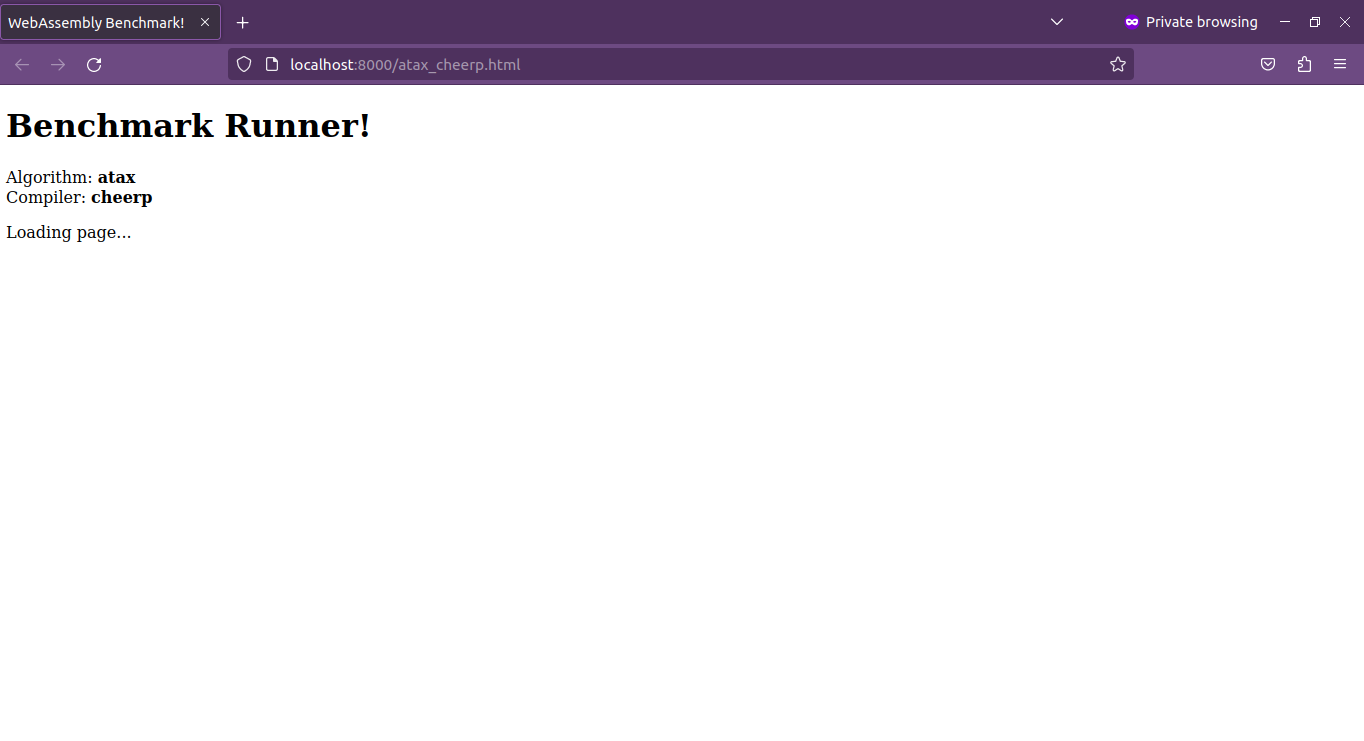
\includegraphics[scale=0.3]{images/html_firefox.png}
    \caption{Arquivo HTML aberto no navegador Firefox para o algoritmo \code{atax}}
    \label{fig:html}
\end{figure}

Na figura é apresentado o texto \textit{Loading page...}, ele permanece por um segundo para certificar-se que o navegador foi inicializado corretamente. Esse texto é alterado automaticamente conforme o experimento progride para informar o pesquisador o estágio que está sendo realizado.
 
\section{Descrição do ambiente}

Foi rodado na máquina do laboratório




\chapter{Resultados}\label{resultados}

No capítulo atual, é apresentado tabelas com os dados coletados, os dados abrangem o tamanho do binário emitido pelos compiladores e quantidade de memória utilizada ao executa-los. Ademais, é apresentado estatísticas descritivas sobre o tempo de execução coletado. Por fim, nesse capítulo é analisado os dados apresentados visando responder as questões de pesquisa formuladas no capítulo inicial.

\section{Análise do tempo de execução}

A análise do tempo de execução será realizada de forma semelhante a análise feita na seção anterior, isto é, para cada tripla(algoritmo, navegador e tamanho de entrada) será calculado a razão entre o tempo de execução apresentado pelo Cheerp sobre o tempo apresentado pelo seu rival.

\begin{longtable}{lrr}\caption{Razões do tempo de execução \label{time_stat_analisys}} \\
\toprule
{} &  Tempo Exec. (entrada grande) &  Tempo Exec. (entrada média) \\
\midrule
\endfirsthead

\toprule
{} &  Tempo Exec. (entrada grande) &  Tempo Exec. (entrada média) \\
\midrule
\endhead
\midrule
\multicolumn{3}{r}{{Continued on next page}} \\
\midrule
\endfoot

\bottomrule
\endlastfoot
Média      &                         1.578 &                        2.095 \\
Desvio p.  &                         0.637 &                        1.009 \\
Min.       &                         0.978 &                        0.778 \\
1° quartil &                         1.043 &                        1.199 \\
2° quartil &                         1.312 &                        2.064 \\
3° quartil &                         1.859 &                        2.915 \\
Max.       &                         3.180 &                        5.000 \\
\end{longtable}


\section{Questões de Pesquisa}

Diante da análise realiza, há informações necessárias para responder as questões de pesquisa enunciadas no capítulo inicial. Portanto, a seguir será respondido cada uma delas, utilizando as conclusões obtidas nesse capítulo.

\begin{description}
    \item[QP01] Qual dos dois compiladores estudados emite um binário com tamanho menor?

    Independente do tamanho da entrada, na média o Cheerp apresentou um binário 10\% menor que o binário emitido pelo Emscripten. Ademais, a variação desse percentual foi muito pequena, logo, em todos os algoritmos utilizados esse resultado se mostrou verdadeiro.

    \item[QP02] Entre os dois, qual produz um binário que utiliza menos memória, considerando o tamanho inicial da memória igual para ambos?
\end{description}



% ----------------------------------------------------------
\chapter{Conclusões}\label{conclusoes}
% ----------------------------------------------------------

Nessa monografia foi realizado uma comparação entre dois compiladores para a plataforma WebAssembly, são os compiladores Cheerp e Emscripten. A pesquisa teve objetivo de comparar a performance das duas ferramentas através de uma análise do tamanho do binário emitido pelos compiladores, do uso de memória e tempo de execução.


\section{Trabalhos futuros}

Tem um monte de coisa para fazer ainda, mas eu quero é meu canudo.



% ----------------------------------------------------------
% ELEMENTOS PÓS-TEXTUAIS
% ----------------------------------------------------------
\postextual
% ----------------------------------------------------------

% ----------------------------------------------------------
% Referências bibliográficas
% ----------------------------------------------------------
\begingroup
    \SingleSpacing\printbibliography[title=REFERÊNCIAS]
\endgroup

% ----------------------------------------------------------
% Glossário
% ----------------------------------------------------------
%
% Consulte o manual da classe abntex2 para orientações sobre o glossário.
%
%\glossary

% ----------------------------------------------------------
% Apêndices
% ----------------------------------------------------------

% ---
% Inicia os apêndices
% ---
\begin{apendicesenv}
	\partapendices* 
	
\chapter{Executável responsável por execução do experimento}\label{run_script}

No Código \ref{run_script_quadro} é apresentado um programa executável escrito na linguagem de programação bash. Após o ambiente estar configurado, este é o programa executado para realizar o experimento. O funcionamento do mesmo é explicado durante o capítulo \ref{delineamento}. Este arquivo também pode ser encontrado no repositório já citado, especificamente no \textit{link} \href{https://github.com/raulpy271/polybench-c-wasm/blob/main/run.sh}{github.com/raulpy271/polybench-c-wasm/blob/main/run.sh}.

\begin{quadro}
\caption{\textit{Script} em bash para execução do experimento\label{run_script_quadro}}
\begin{lstlisting}[tabsize=2, basicstyle=\ttfamily\tiny]
#!/bin/bash

FIREFOX=firefox
CHROME=google-chrome-stable
DOWNLOAD_DIR="$HOME/Downloads"
FULL_BENCHMARK="$DOWNLOAD_DIR/benchmark_full.csv"

CATEGORIES=(
    'linear-algebra/blas'
    'linear-algebra/kernels'
    'linear-algebra/solvers'
    'datamining'
    'stencils'
    'medley'
)

run_each_algorithm () {
    for category in ${CATEGORIES[@]};
    do
        curr_pwd=`pwd`
        algorithms=`ls $category`
        for algorithm in $algorithms;
        do
            benchmark_path=$category/$algorithm
            echo "Entering $benchmark_path"
            cd $benchmark_path
            make -s clean
            make -s
            echo "Running benchmark"
            python3 -m http.server &> /dev/null &
            $FIREFOX --private-window http://localhost:8000/${algorithm}_cheerp.html &> /dev/null
            $FIREFOX --private-window http://localhost:8000/${algorithm}_emscripten.html &> /dev/null
            $CHROME --incognito http://localhost:8000/${algorithm}_cheerp.html &> /dev/null
            $CHROME --incognito http://localhost:8000/${algorithm}_emscripten.html &> /dev/null
            echo "Benchmark runned."
            kill `pidof -s python3`
            cd $curr_pwd
        done
    done
}

create_full_benchmark_result () {
    benchmark_files=(`ls $DOWNLOAD_DIR/benchmark_*`)
    # Create CSV Header
    head -n 1 ${benchmark_files[0]} > $FULL_BENCHMARK
    # Create CSV Body
    tail -q -n +2 ${benchmark_files[@]} >> $FULL_BENCHMARK
}

run_each_algorithm
echo "Crating full CSV"
create_full_benchmark_result
echo $FULL_BENCHMARK " created!"
\end{lstlisting}
\end{quadro}

	\chapter{Compilação utilizando \code{Makefile}}\label{makefile}

Este apêndice apresenta o Código \ref{makefile_quadro}, onde há um exemplo de arquivo no formato \code{Makefile} utilizado para realizar compilação para WebAssembly dos algoritmos do PolyBench/C. Este exemplo é utilizado para compilar o algoritmo \code{atax} do PolyBench/C, no entanto, é gerado automaticamente arquivos semelhantes para compilar os outros algoritmos presentes no \textit{benchmark}.

Este arquivo foi gerado automaticamente por um \textit{script} responsável por emitir um \code{Makefile} para cada algoritmo. Esse \textit{script} pode ser visto no endereço \href{https://github.com/raulpy271/polybench-c-wasm/blob/main/wasm-makefile-gen.py}{github.com/raulpy271/polybench-c-wasm/blob/main/wasm-makefile-gen.py}. Ademais, os parâmetros de compilação utilizados no Código \ref{makefile_quadro} são descritos na seção.

\begin{quadro}
\caption{Exemplo de arquivo \code{Makefile} para compilação do algoritmo \code{atax}\label{makefile_quadro}}
\begin{lstlisting}[tabsize=2, basicstyle=\ttfamily\tiny]
CHEERP=/opt/cheerp/bin/clang
EMCC=emcc
DATASET_SIZE=MEDIUM_DATASET
CHEERP_FLAGS=-O2 -cheerp-pretty-code -target cheerp-wasm \
	-cheerp-linear-heap-size=2000 -cheerp-make-module=es6
EMCC_FLAGS=-O2 --minify 0 -sINITIAL_MEMORY=1114112 -sALLOW_MEMORY_GROWTH \
	-sMAXIMUM_MEMORY=$$((2000 * 1024 * 1024))
POLYBENCH_FLAGS=-DPOLYBENCH_TIME -D$(DATASET_SIZE)

.PHONY: all clean

all: atax_cheerp.mjs atax_cheerp.html atax_emscripten.mjs atax_emscripten.html

atax_cheerp.wasm atax_cheerp.mjs: atax.c atax.h
	$(CHEERP) $(CHEERP_FLAGS) $(POLYBENCH_FLAGS) \
		-I /home/raul/ccicomp/tcc/polybench-c-4.2.1-beta/utilities -I . \
        /home/raul/ccicomp/tcc/polybench-c-4.2.1-beta/utilities/polybench.c atax.c \
		-o atax_cheerp.mjs
	cat /home/raul/ccicomp/tcc/polybench-c-4.2.1-beta/utilities/cheerp_capture_time.js >> atax_cheerp.mjs
	# Store initial size of the heap
	sed -E -i '/function\s+__start\s*\(/a initial_memory = __heap.byteLength;' atax_cheerp.mjs
	# Store final size of the heap and return result
	sed -E -i \
		'/^\s*__start\s*\(\s*\)/a memory_used = __heap.byteLength; \
		return {polybench_time, initial_memory, memory_used};' \
		atax_cheerp.mjs

atax_emscripten.wasm atax_emscripten.mjs: atax.c atax.h
	$(EMCC) $(EMCC_FLAGS) $(POLYBENCH_FLAGS) \
		-I /home/raul/ccicomp/tcc/polybench-c-4.2.1-beta/utilities -I . \
		/home/raul/ccicomp/tcc/polybench-c-4.2.1-beta/utilities/polybench.c atax.c \
		--post-js /home/raul/ccicomp/tcc/polybench-c-4.2.1-beta/utilities/emscripten_capture_time.js \
		-o atax_emscripten.mjs

atax_cheerp.html: /home/raul/ccicomp/tcc/polybench-c-4.2.1-beta/utilities/runner.template.html
	sed 's/$$ALGORITHM/atax/;s/$$COMPILER/cheerp/;s/$$DATASET_SIZE/$(DATASET_SIZE)/' \
		/home/raul/ccicomp/tcc/polybench-c-4.2.1-beta/utilities/runner.template.html > atax_cheerp.html

atax_emscripten.html: /home/raul/ccicomp/tcc/polybench-c-4.2.1-beta/utilities/runner.template.html
	sed 's/$$ALGORITHM/atax/;s/$$COMPILER/emscripten/;s/$$DATASET_SIZE/$(DATASET_SIZE)/' \
		/home/raul/ccicomp/tcc/polybench-c-4.2.1-beta/utilities/runner.template.html > atax_emscripten.html

clean:
	@ rm -f atax*.mjs atax*.wasm atax*.html
\end{lstlisting}
\end{quadro}


\end{apendicesenv}
% ---


% ----------------------------------------------------------
% Anexos
% ----------------------------------------------------------

% ---
% Inicia os anexos
% ---
%\begin{anexosenv}
%%	\partanexos*
%	\input{aftertext/anexo_a}
%\end{anexosenv}

%---------------------------------------------------------------------
% INDICE REMISSIVO
%---------------------------------------------------------------------
%\phantompart
%\printindex
%---------------------------------------------------------------------

\end{document}
